\begin{figure}[t]\centering
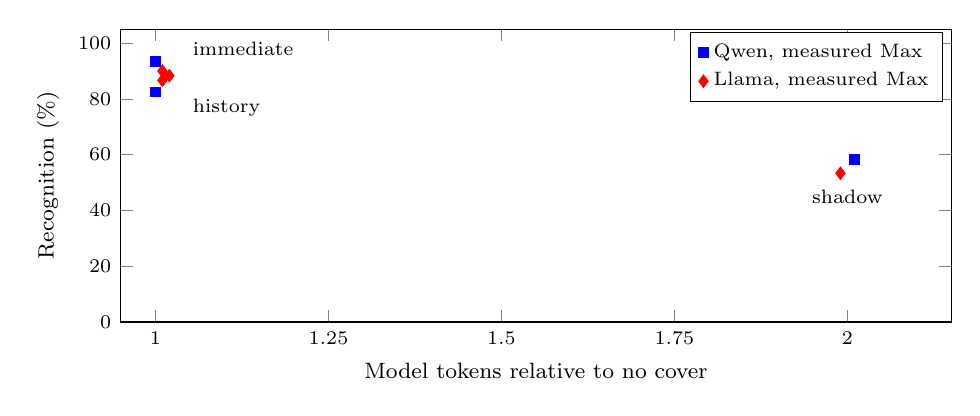
\begin{tikzpicture}
\begin{axis}[width=\columnwidth,height=5.3cm,xmin=0.95,xmax=2.15,ymin=0,ymax=105,
 xlabel={Model tokens relative to no cover},ylabel={Recognition (\%)},
 xtick={1,1.25,1.5,1.75,2},ytick={0,20,40,60,80,100},
 legend style={font=\scriptsize,at={(0.99,0.99)},anchor=north east,cells={anchor=west}},
 tick label style={font=\scriptsize},label style={font=\footnotesize}]
\addplot[only marks,blue,mark=square*,mark size=1.7pt] coordinates {(1,93.33) (1,82.5) (1,82.5) (2.01,58.33)};
\addlegendentry{Qwen, measured Max}
\addplot[only marks,red,mark=diamond*,mark size=2.2pt] coordinates {(1.01,90) (1.01,86.67) (1.02,88.33) (1.99,53.33)};
\addlegendentry{Llama, measured Max}
\node[font=\scriptsize,anchor=west] at (axis cs:1.04,98) {immediate};
\node[font=\scriptsize,anchor=west] at (axis cs:1.04,77) {history};
\node[font=\scriptsize,anchor=north] at (axis cs:2,51) {shadow};
\end{axis}
\end{tikzpicture}
\caption{Measured recognition and model work for the four cover policies. Points are strongest tested call-window attacks; overlapping controller points retain their values. Shadow changes call count and composition as well as model work. Ideal candidate-label values are shown separately in Table~\ref{tab:shadow-floor}.}\label{fig:frontier}
\end{figure}
